\documentclass[a4paper]{article}

%% Language and font encodings
\usepackage[english]{babel}
\usepackage[utf8x]{inputenc}
\usepackage[T1]{fontenc}

%% Sets page size and margins
\usepackage[a4paper,top=3cm,bottom=2cm,left=3cm,right=3cm,marginparwidth=1.75cm]{geometry}

%% Useful packages
\usepackage{amsmath}
\usepackage{graphicx}
\usepackage[colorinlistoftodos]{todonotes}
\usepackage[colorlinks=true, allcolors=blue]{hyperref}

\title{ECE 276A Homework 2: Orientation Tracking}
\author{Samuel Bauza A10025697}

\begin{document}
\maketitle

\section{Introduction}

	Orientation Tracking is used in a wide range of fields from robotics to object tracking to mobile devices. All modern smart-phones, robots and many camera systems include orientation tracking to improve user experience, localization, or provide other pertinent data to the system.

	Many of these systems use simple force measuring devices, such as accelerometers, gyroscopes and magnetometers, which are all prone to inducing error. Some form of merging the measurements from each of these devices in needed to improve the accuracy of the estimated orientation.
    
    This project explores one method of estimating orientation using an Unscented Kalman Filter (UKF). Its accuracy is compared to ground truth (measured using a vicon system), and it is used alongside image data to produce a large panorama image.

\section{Problem Formulation}

	We are given several data sets, each of which contains a series of time-stamped IMU data points. Some sets also include ground-truth vicon data collected from a separate imaging system, and image data, collected from a camera attached to the IMU. The primary goal of this project is to provide an accurate orientation estimate over time by merging the accelerometer and gyroscope data provided by the IMU. A secondary goal is to use this orientation estimate to create a panorama using image data when it is present.

This problem contains three parts: Data Normalization, Orientation Estimation, and Panorama Generation. Data Normalization is the process of taking the IMU data and converting it to recognizable units, specifically g's and degrees from each axis. Orientation estimation takes the force and rotational velocity measurements and passes them through an Unscented Kalman Filter, which should improve the estimation accuracy given noisy measurements. Panorama Generation takes the orientation estimates and image data to place each image on a sphere, which is later flattened to produce the final panorama.
	The math and assumptions behind data normalization are pretty simple. The system is assumed to be stationary for the first few seconds. The accelerometer and gyroscope bias can be collected by subtracting the mean of these samples from the zero point (below), which can be determined, along with the device sensitivity by looking at the relevant data sheet\ref{IMU_ref}.
    
\begin{equation*}\label{eq:sensa_bias}
sensitivity_a = \frac{3.3 V}{1023} * \frac{1}{.30}
\end{equation*}
\begin{equation*}\label{eq:sensg_bias}
sensitivity_g = \frac{3.3 V}{1023} * \frac{1}{330}
\end{equation*}
\begin{equation*}\label{eq:accel_bias}
accelerometerbias = \sum{[Fx,Fy,Fz]} - [512,512,512 + 1 / sensitivity_a]
\end{equation*}
\begin{equation*}\label{eq:gyro_bias}
gyrobias			=\sum{[Fx,Fy,Fz]} - [512,512,512]
\end{equation*}
    
    The Unscented Kalman filter is broken down into multiple stages, namely the prediction and update stages \ref{fig:kalman_eq}. The prediction stage uses one type of data to estimate the future state, while the update state uses other data to update to a "true" state. In this case, it is used to decrease the drift caused by integrating gyroscope values.
    
\begin{figure}[h]
  \centering
    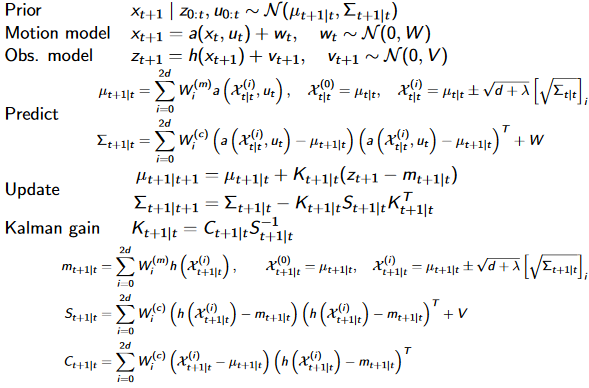
\includegraphics[width=1\textwidth]{kalman_eq.png}
  \caption{Kalman update equations\label{fig:kalman_eq}}
\end{figure}
    
    Finally, the panorama involves several mappings from spherical to cylindrical and spherical to Cartesian transforms, which use the following equations:
    
\begin{equation*}
\rho = \sqrt[2]{x^2 + y^2 + z^2}
\end{equation*}
\begin{equation*}
\theta = arccos(\frac{z}{r})
\end{equation*}
\begin{equation*}
\phi = arctan(\frac{y}{x})
\end{equation*}
\begin{equation*}
x = \rho * sin(\phi) * cos(\theta)
\end{equation*}
\begin{equation*}
y = \rho * sin(\phi) * sin(\theta)
\end{equation*}
\begin{equation*}
z = \rho * cos(\phi)
\end{equation*}

\section{Technical Approach}

	The steps taken are discussed in greater detail below. Note that only training sets contain ground truth (vicon) data, and that not all data sets contain image data for panorama generation. Panoramas for which image data is available are presented.

\subsection{Orientation Formats}

	There are several different methods of representing an orientation in 3D space: namely Euler angles, Rotation Matrices and Quaternions. Euler angles, i.e. roll, pitch, yaw, are generally easy to visualize, but can be tricky to deal with mathematically. Rotation matrices largely suffer from the same problems as Euler angles. Finally, Quaternions are difficult to visualize, but are do not suffer from the same mathematical issues that Euler angles and rotation matrices suffer from.

\subsubsection{Euler Angles}

As mentioned above, Euler angles (Figure \ref{fig:euler_im}) are the roll, pitch, and yaw measurements used to calculate orientation. More specifically, they are the rotations about the x-y-z axis respectively. Most people generally find these easy to visualize, but they can be difficult to manipulate. In particular, there are discontinuities in the measurement space, i.e. a measurement of $\pi$ radians rolls over to -$\pi$ and -$\pi$ = $\pi$. This can generally make it difficult to average, interpolate between values and generally handle multiple rotations.

\begin{figure}[h]
  \centering
    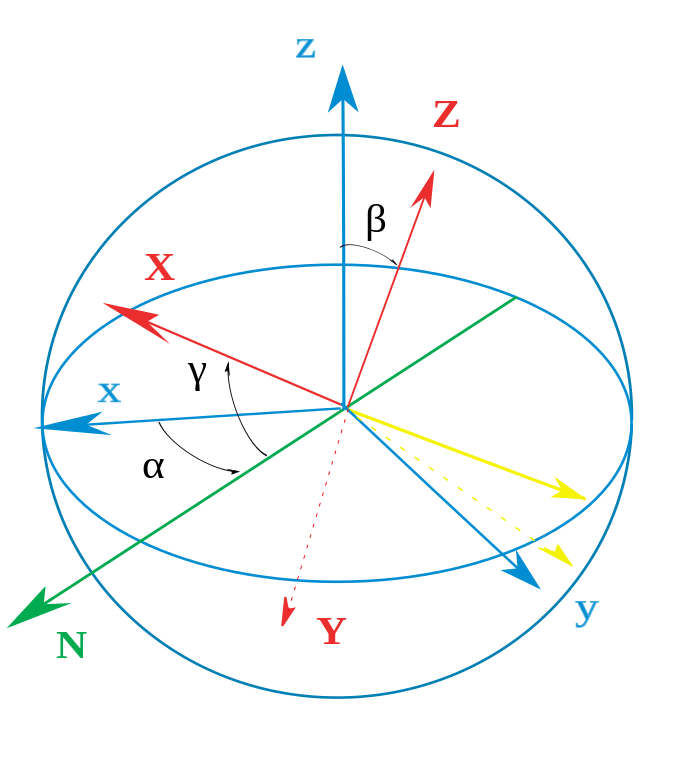
\includegraphics[width=.5\textwidth]{euler_im.png}
  \caption{Visual Description of Euler Angles\label{fig:euler_im}}
\end{figure}

\subsubsection{Rotation Matrices}

	Another method of representing an orientation is to use rotation matrices (Figure \ref{fig:rot_mat}). These can be easily used to transform Cartesian coordinates using matrix multiplication. This is the format vicon data comes in. These make the addition of multiple rotations much easier to perform than when directly using Euler angles, but suffers from the same discontinuity problems that Euler angles do.
\begin{figure}[h]
  \centering
    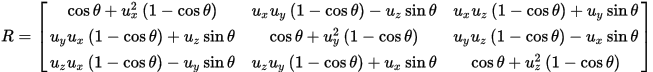
\includegraphics[width=1\textwidth]{rot_mat.png}
  \caption{Rotation Matrix Equations\label{fig:rot_mat}}
\end{figure}

\subsubsection{Quaternions}

Yet another method of representing a rotation comes in the form of a quaternion. Quaternions are a 4-term object, with a scalar term qw, and a three-component vector <Rx,Ry,Rz>. This is often represented as <qw,qx,qy,qz>, though distinctions are made during calculations. Though these are more difficult to visualize, they make many mathematical operations much simpler. A comprehensive list of quaternion manipulations is in Figure \ref{fig:quat_eq}.

\begin{figure}[h]
  \centering
    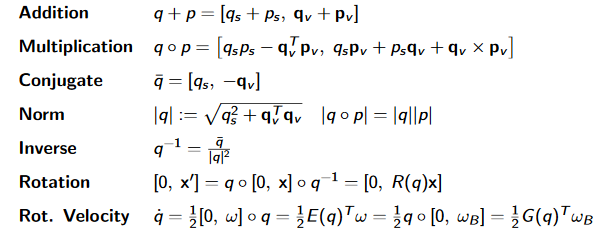
\includegraphics[width=1\textwidth]{quat_eq.png}
  \caption{Various Quaternion Functions\label{fig:quat_eq}}
\end{figure}

\begin{equation*}\label{eq:eul2quat}
<qw,qx,qy,qz> 	= e^{qs} * [cos(||q_v||),\frac{q_v}{||q_v||} * sin(||q_v||)]
\end{equation*}
\begin{equation*}\label{eq:quat2eul}
<0,Rx,Ry,Rz>		= 2 *[ln(|q|),\frac{q_v}{||q_v||}*arccos(\frac{q_v}{||q_v||})]
\end{equation*}

\subsection{IMU Data Normalization}

The first step in estimating the orientation is to collect the data from the Inertial Measurement Unit (IMU) \cite{IMU}. The values from the devices are voltage measurements. In order to get sensible information out of it, these values must be converted to force and rotational velocities. First, the value of each voltage delta must be determined, which is then used to estimate the bias. Each device is effected by a measurement bias that can change with temperature and time, so it must be estimated at run time.

\subsubsection{Bias and Sensitivity Estimation}

The device manual is used to determine what sensitivity values and data resolution to use. In our case, both devices use a 10-bit ADC, centered at 512. The accelerometer has a sensitivity of $\frac{3g}{Volt}$ while the gyroscope has a sensitivity of $\frac{333 degrees}{second * Volt}$. These are used in the bias equations above.

At rest a force of [0,0,1] is felt by the accelerometer, and no rotation is experienced by the gyroscope. Furthermore, it is assumed that the first few seconds of each run are stationary,With these assumptions bias equations (above) can be used to estimate the bias of each device. These bias values will change dataset to dataset.

\subsubsection{Gyroscope Integration}

One Naive method of estimating orientation would be to simply integrate the rotational velocities over time. In our case, the rotational velocities are converted to a quaternion which is integrated. If the initial position is known, it can be added to the integration estimate. This will work for short periods of time, but because of the finite sample rate error will immediately begin to accumulate in the integration, causing the estimate to drift over time. Because of this a better method will be needed

\subsection{Unscented Kalman Filtering}

	The Unscented Kalman filter is a non-linear variant of the typical Kalman filter \cite{KRAFT}. It operates by using one set of information, in this case gyroscope data, to predict its state (orientation), then updating the actual state using another set of data (accelerometer). In doing so, it keeps track of mean and covariance statistics for the input data, and prediction errors. This tends to improve the prediction ability, and should account for gyroscope drift.
    
Some relevant terms:

$E_t^{(i)}$ = Forward error terms

$q_{t+1|t}^{i}$ = Predicted State

$P_{t+1|t}$ = State Covariance

Q = Process Covariance

$e_t^{(i)}$ = error vectors (from quaternion averaging)

$\alpha$ =	quaternion weights

$z_{t+1}$ = Observation model output

g = $[0,0,1]^T$ gravity vector

$\alpha_{cov}$ = Covariance weights

$P_{zz}$ = weighted outer product of acceleration

$P_R$ = measurement noise

$P_{xz}$ = cross correlation

$P_{t+1|t+1}$ = Predicted State

$q_{t+1|t+1}$ = updated state

$K_{t+1}$ = Kalman gain

\subsubsection{Initialization}

On startup, values for the initial state, Process covariance, and measurement noise are set to initial values. This will cause transient effects initially, but these will quickly dissipate as data is entered into the filter.

The state $q_{0|0}$ is initialized as [0,0,0,1]

Process Covariance Q is initialized as .001 * $I^7$.

Measurement noise $P_R$ is initialized as .1 * $I^7$.

\subsubsection{Prediction step}

The prediction step takes in the in the gyroscope integration value and use this to predict the true orientation. This involves collecting expected sigma values from the process covariance and state covariance, and taking the expectation of each of these. This helps correct the prediction given the gyro input.

$E_t^{(i)}$ = columns((0,0,0),$\pm$sqrt(6*$P_{t|t} + Q$))

$q_{t+1|t}^{(i)} = q_{t|t} \circ exp([0,.5*E_t^{(i)}]) \circ exp([0,.5 * \omega _t \delta t])$

$q_{t+1}^{mean} = avg(q_{t+1|t}^{(i)},\alpha ^{(i)})$

$P_{t+1|t} = \sum{\alpha ^{(i)} * e_{t+1|t}^\circ * e_{t+1|t}^{(i) T}}$

$e_{t+1|t}^{(i) T}$ comes from the average function

\subsubsection{Update Step}

The update step uses the 'true' state to update the process and error covariances, which are used in the prediction step. The output in our case should be used to generate the panoramas later in the process.

$[0,z_{t+1}^{(i)}] = q_{t+1|t}^{(i)} \circ [0,g]^T \circ q_{t+1|t}^{-(i)}$

$z_{t+1}^{mean} = \sum{z_{t+1}^{(i)} * \alpha ^{(i)}}$

$P_{zz} = \sum{ [( z_{t+1}^{(i)} - z_{t+1}^{mean})^2] * \alpha_{cov}^{(i)}}$

$P_{vv} = P_{zz} + P_R$

$P_{xz} = \sum{E_t^{(i)}( z_{t+1}^{(i)} - z_{t+1}^{mean}) * \alpha ^{(i)}}$

$K_{t+1} = P_{xz} * P_{vv}^{-1}$

\subsection{Panorama Generation}

After the orientation over time is estimated, image data can be used to generate a panorama. This is done in several stages: First the Cartesian coordinate of each pixel in the body frame is calculated using the known image focal length and dimensions. For each image, the estimated orientation at that time is used to rotate each of these coordinates from the body frame into the world frame. These new coordinates are changed back into spherical coordinates, then projected onto the final panoramic image. As new images are loaded in, pixels drawn by previous images are overwritten.

\subsubsection{Body Frame Generation}

In our case, each image represented a 60$^{\circ}$ wide by 45$^{\circ}$ tall focal length, with a width and height of 320 and 240 pixels respectively. In spherical coordinates, this means that the $\theta$ spans -30$^{\circ}$ < $\theta$ < 30$^{\circ}$ and $\phi$ spans 67.5$^{\circ}$ < $\phi$ <  112.5$^{\circ}$. The radius of the sphere $\rho$ is assumed to be 1. The body frame of each image shares these spherical coordinates, so they can be converted into Cartesian coordinates before processing.

\subsubsection{World Frame Conversion}

We can now collect the time stamp for each image, and calculate the resulting pixel locations in the world frame. This is done simply using a quaternion rotation on each Cartesian coordinate. Numpy enables this calculation to be done without using loops.

\subsubsection{Cylindrical Projection}

The new Cartesian coordinates can now be converted back into spherical coordinates (above), and because it was rotated by a union quaternion, all rho values should still be 1. To project the spherical coordinates onto a cylinder use the following equations. Note that r is not calculated, this is because r is again assumed to be 1. At this point, the values in the resulting array represent the z and $\theta$ values of each image pixel index, mapping the image onto the panorama. This projection has the effect of stretching all pixels near the poles across the resulting panorama, while maintaining resolution near the center row of the image.

\begin{equation*}
z = \rho * cos(\phi)
\end{equation*}
\begin{equation*}
\theta = \theta
\end{equation*}

The results collected from the above process are enumerated below. The panoramas generated from the ground truth data look fairly decent. A problem occurs during some runs when the images are translated through space. All of the above processes assume no translation occurs during data collection, and this translation causes the center of the panorama to become distorted. Several examples of this issue are included, as well as results when these problematic images are removed.

\subsection{Training Set Orientation Estimates}

The training set graphs are included from image \ref{fig:rpy_trainset1} - \ref{fig:rpy_trainset9} Each graph includes the vicon "Ground Truth", the estimated orientation using integration, and the estimated orientation using the Kalman filter. In most cases, the kalman filter is a great improvement over the integrated estimate, though both seem  to suffer from random variations during processing. In many cases, however, the Kalman filter closely matches the ground truth.

Pitch generally functions the best, and roll is often very good, however yaw seems to suffer from random offsets that may be caused by the input state. Accelerometers have difficulty estimating yaw when flat, and so this effect may have caused the Kalman filter to mispredict, particularly when the platform was flat.

\subsection{Test Set Orientation Estimates}

The test set graphs are included from image \ref{fig:rpy_testset10} - \ref{fig:rpy_testset13}, and have comparable performance to the training set. Because Vicon data was not provided, only the integration estimate and Kalman estimates are shown.

\begin{figure}[h]
  \centering
    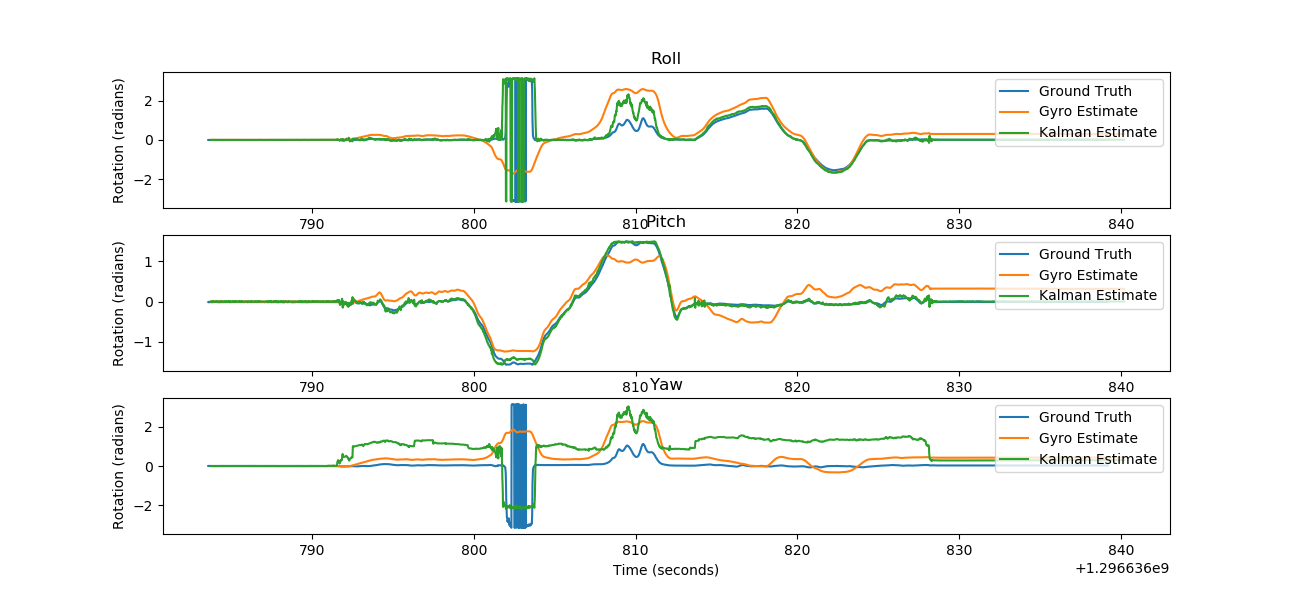
\includegraphics[width=1\textwidth]{rpy_trainset1.png}
  \caption{Estimated orientation over time (Training 1)\label{fig:rpy_trainset1}}
\end{figure}

\begin{figure}[h]
  \centering
    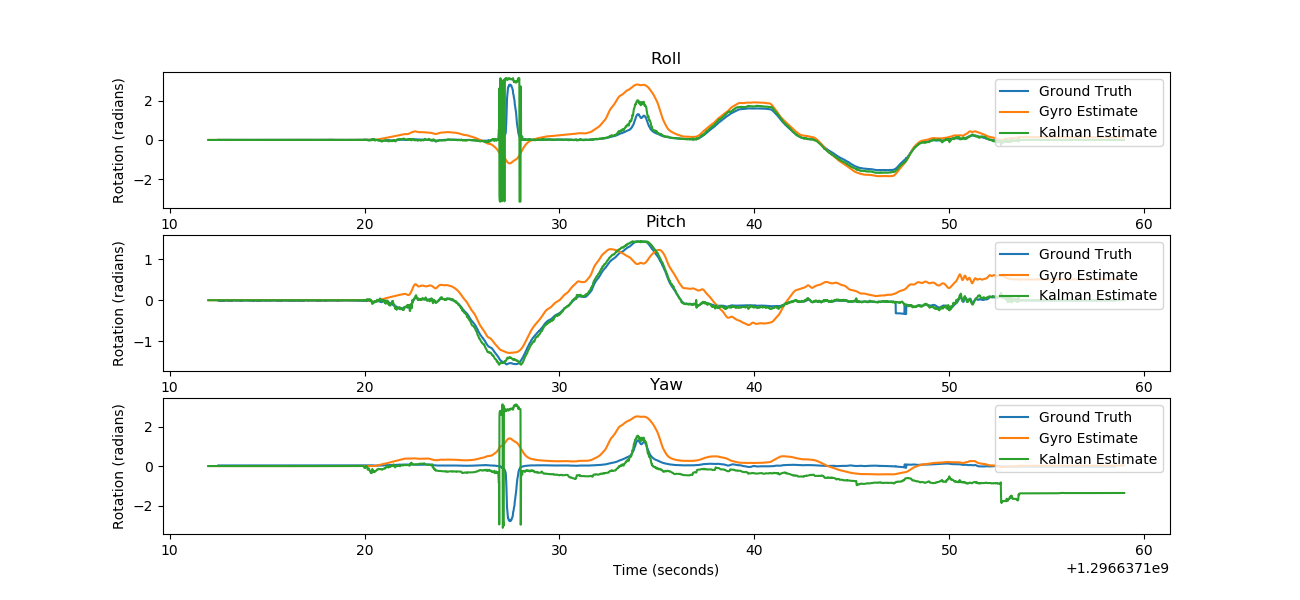
\includegraphics[width=1\textwidth]{rpy_trainset2.png}
  \caption{Estimated orientation over time (Training 2)\label{fig:rpy_trainset2}}
\end{figure}

\begin{figure}[h]
  \centering
    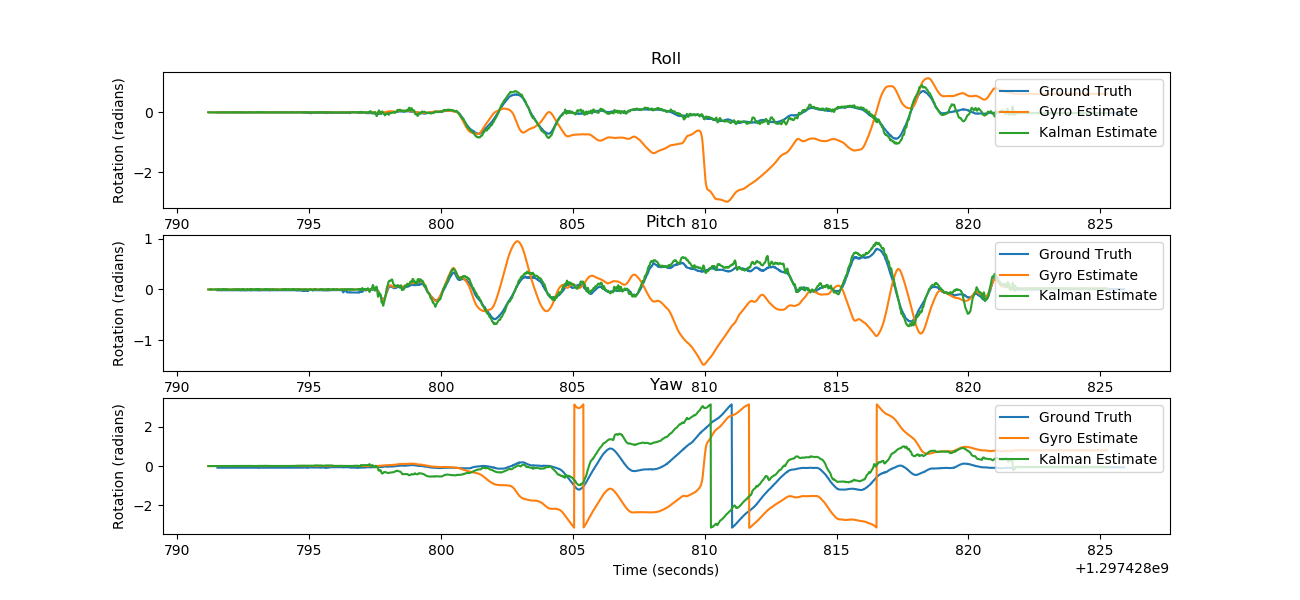
\includegraphics[width=1\textwidth]{rpy_trainset3.png}
  \caption{Estimated orientation over time (Training 3)\label{fig:rpy_trainset3}}
\end{figure}

\begin{figure}[h]
  \centering
    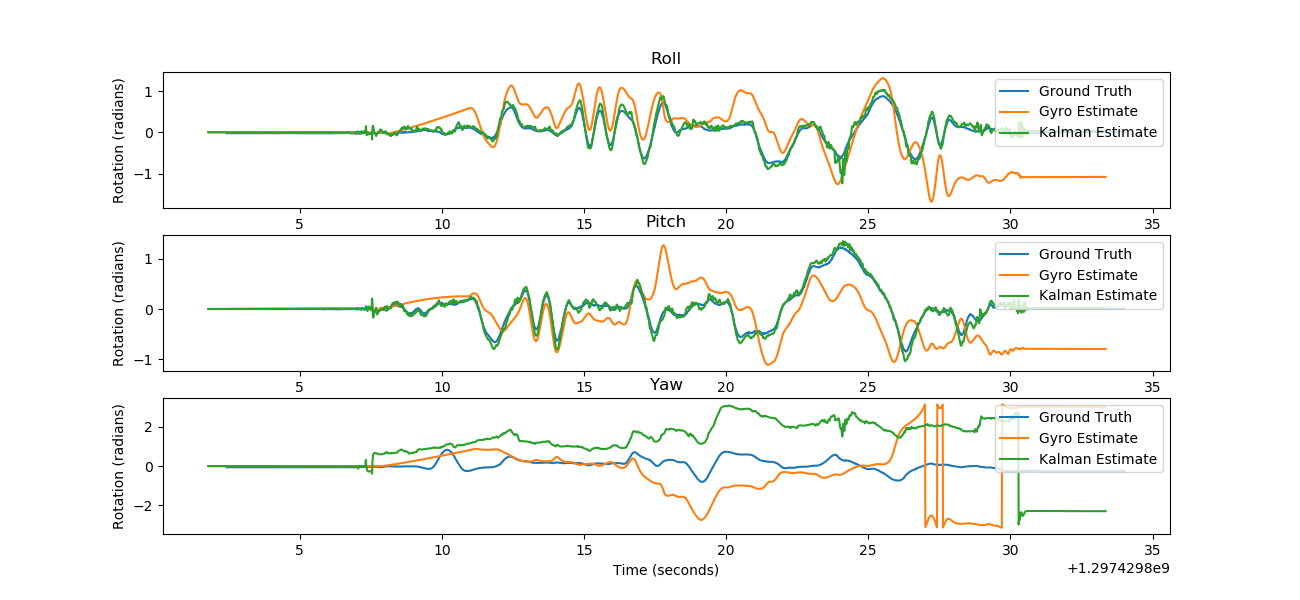
\includegraphics[width=1\textwidth]{rpy_trainset4.png}
  \caption{Estimated orientation over time (Training 4)\label{fig:rpy_trainset4}}
\end{figure}

\begin{figure}[h]
  \centering
    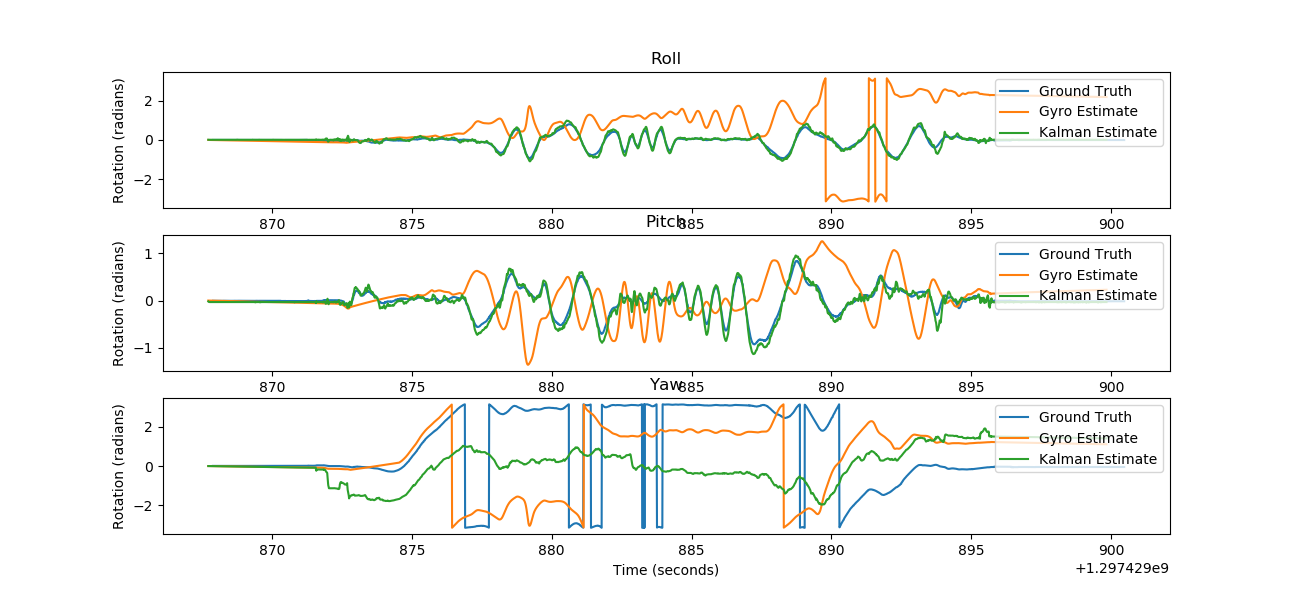
\includegraphics[width=1\textwidth]{rpy_trainset5.png}
  \caption{Estimated orientation over time (Training 5)\label{fig:rpy_trainset5}}
\end{figure}

\begin{figure}[h]
  \centering
    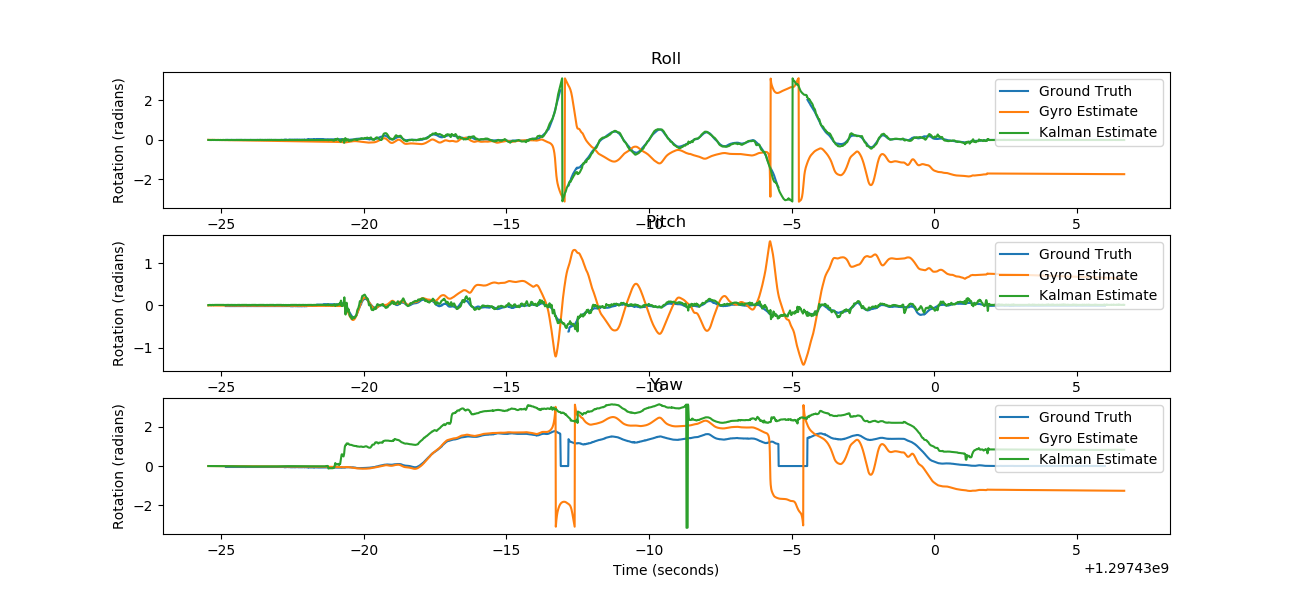
\includegraphics[width=1\textwidth]{rpy_trainset6.png}
  \caption{Estimated orientation over time (Training 6)\label{fig:rpy_trainset6}}
\end{figure}

\begin{figure}[h]
  \centering
    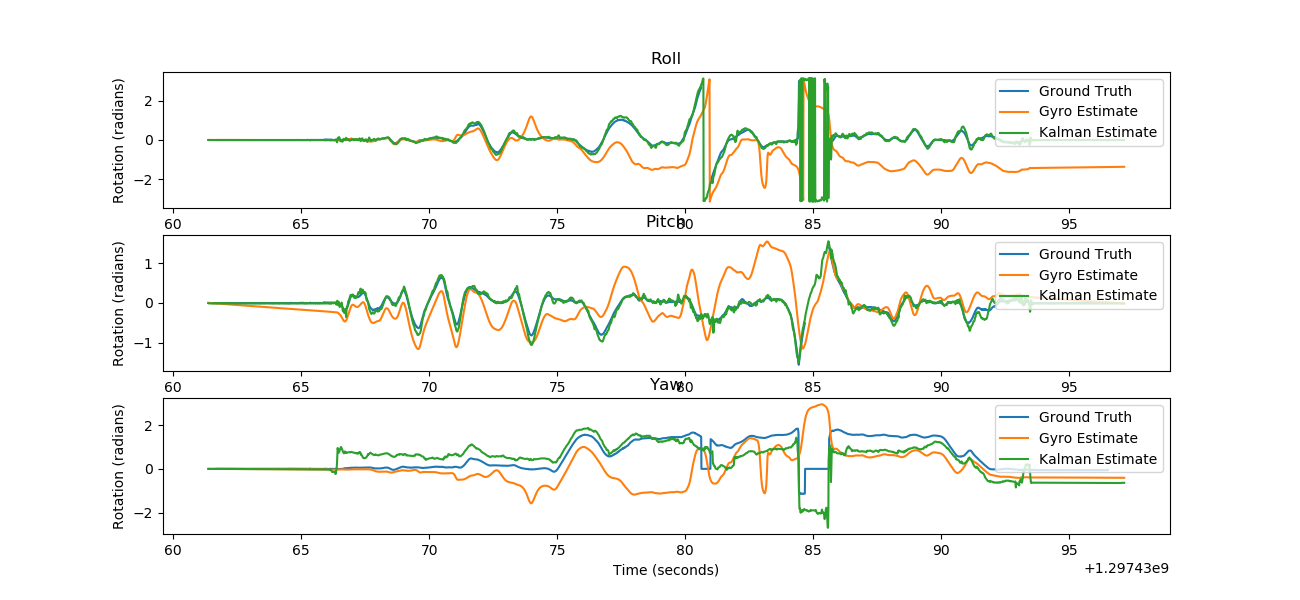
\includegraphics[width=1\textwidth]{rpy_trainset7.png}
  \caption{Estimated orientation over time (Training 7)\label{fig:rpy_trainset7}}
\end{figure}

\begin{figure}[h]
  \centering
    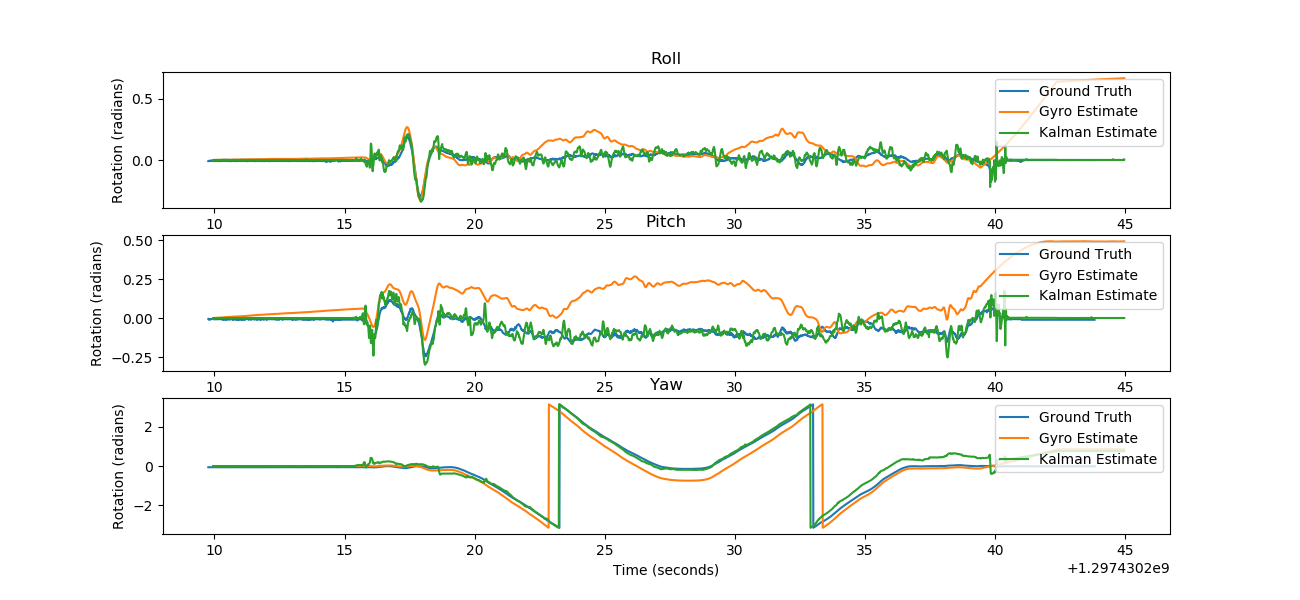
\includegraphics[width=1\textwidth]{rpy_trainset8.png}
  \caption{Estimated orientation over time (Training 8)\label{fig:rpy_trainset8}}
\end{figure}

\begin{figure}[h]
  \centering
    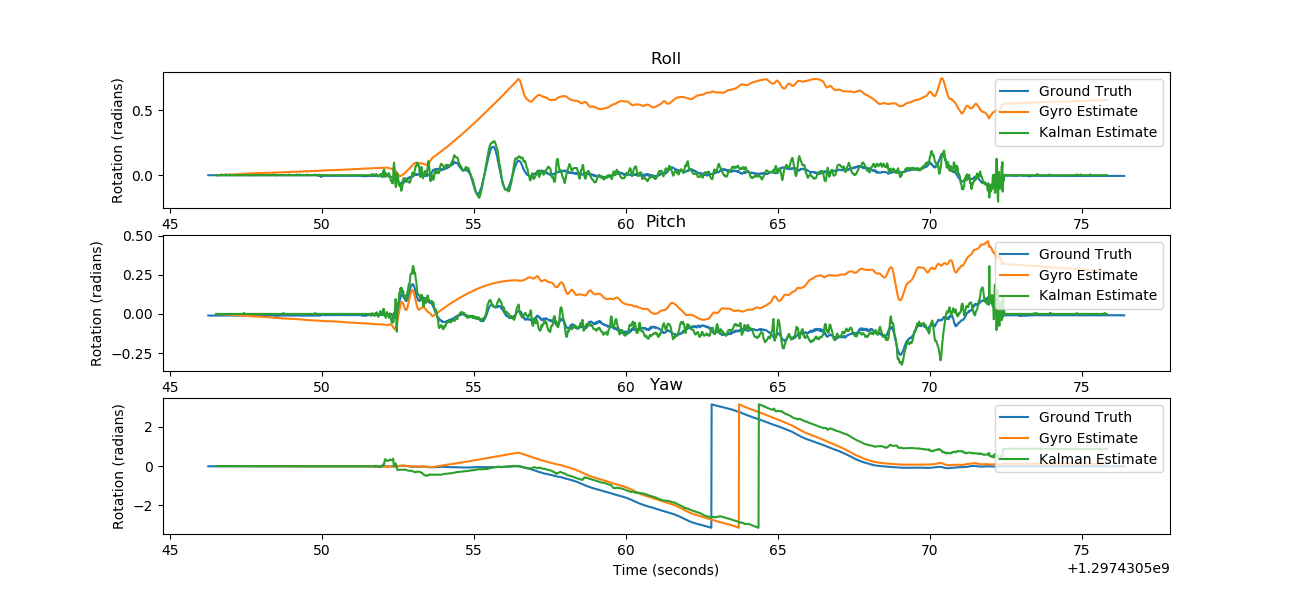
\includegraphics[width=1\textwidth]{rpy_trainset9.png}
  \caption{Estimated orientation over time (Training 9)\label{fig:rpy_trainset9}}
\end{figure}

\begin{figure}[h]
  \centering
    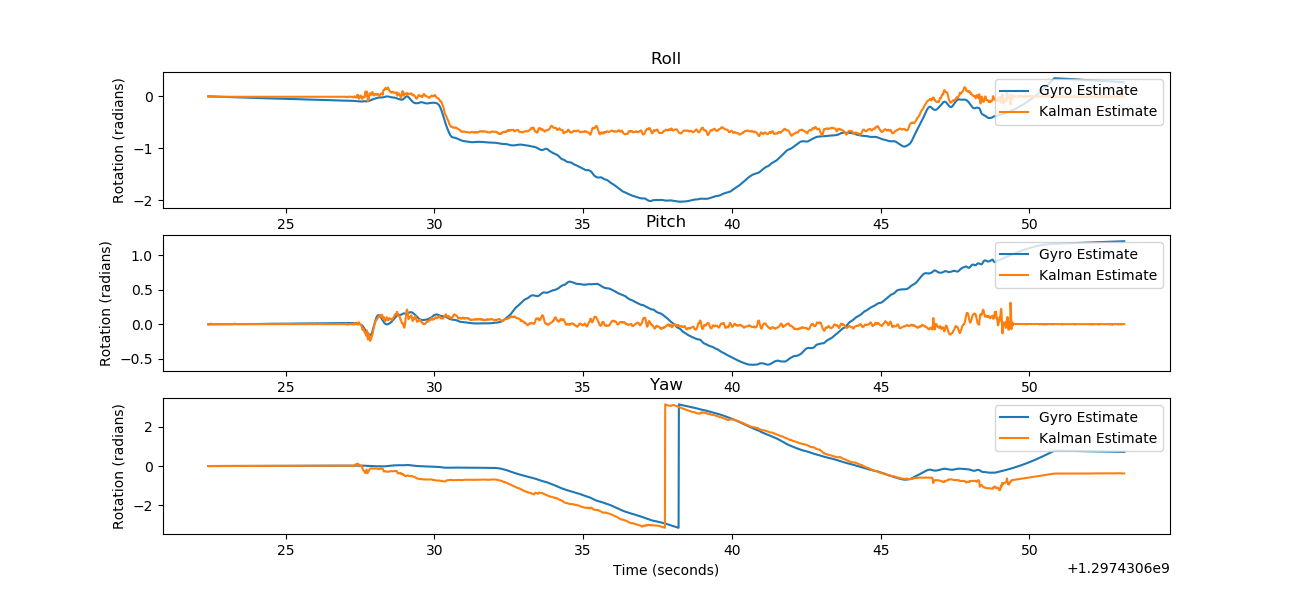
\includegraphics[width=1\textwidth]{rpy_testset10.png}
  \caption{Estimated orientation over time (Test 10)\label{fig:rpy_testset10}}
\end{figure}

\begin{figure}[h]
  \centering
    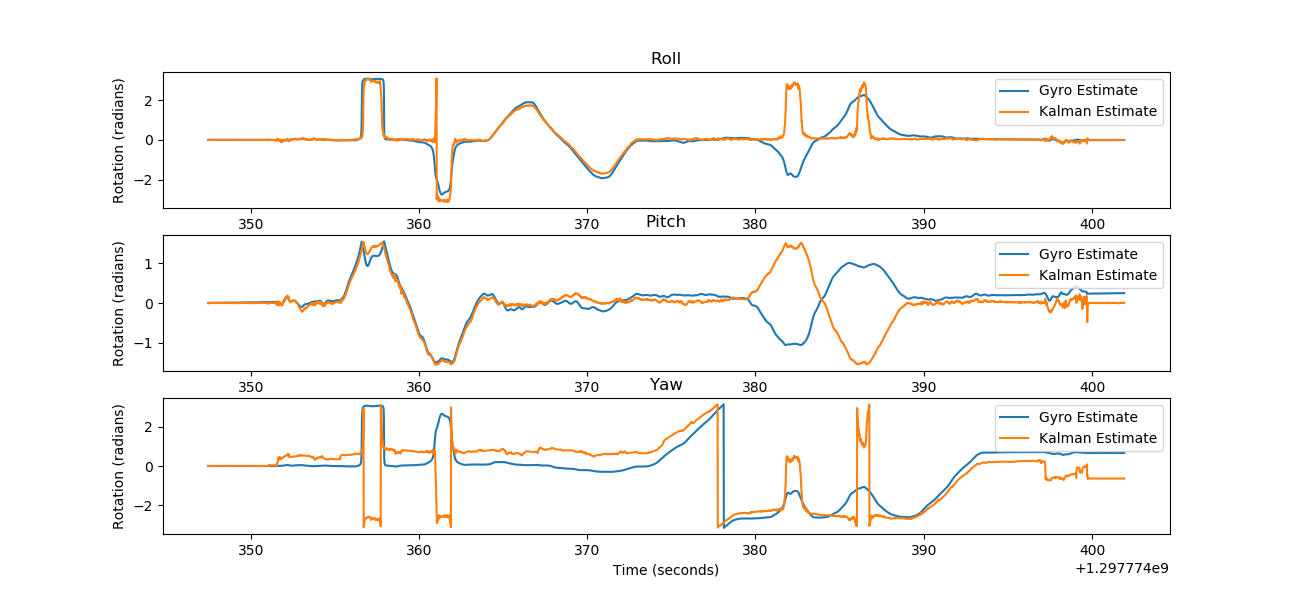
\includegraphics[width=1\textwidth]{rpy_testset11.png}
  \caption{Estimated orientation over time (Test 11)\label{fig:rpy_testset11}}
\end{figure}

\begin{figure}[h]
  \centering
    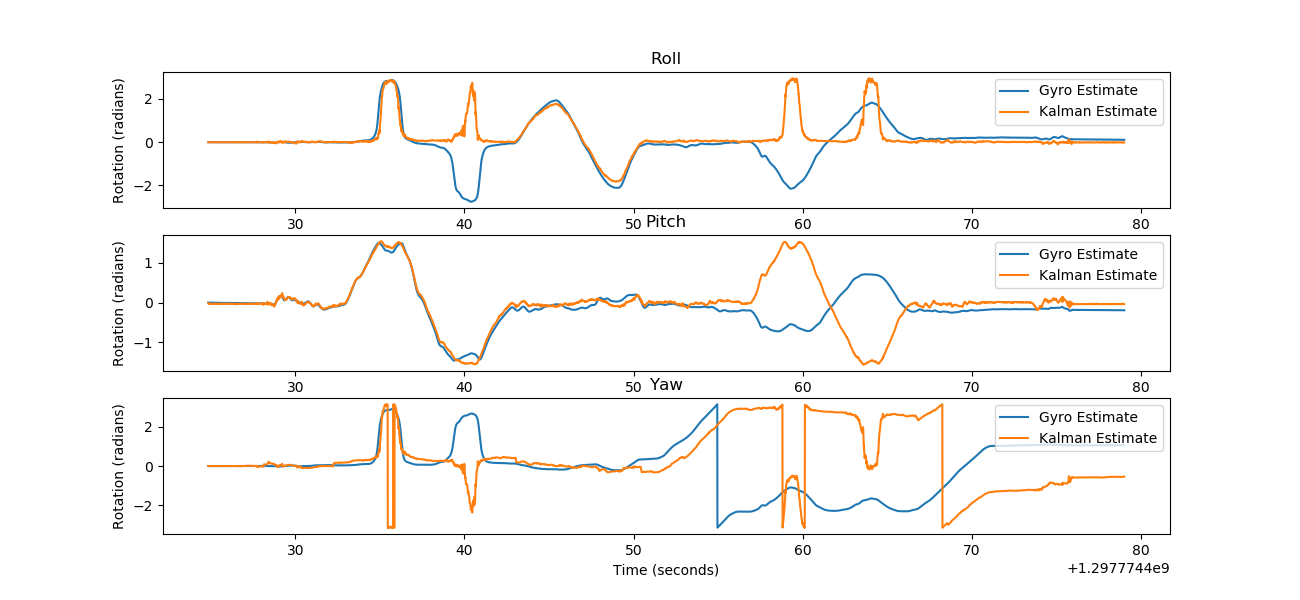
\includegraphics[width=1\textwidth]{rpy_testset12.png}
  \caption{Estimated orientation over time (Test 12)\label{fig:rpy_testset12}}
\end{figure}

\begin{figure}[h]
  \centering
    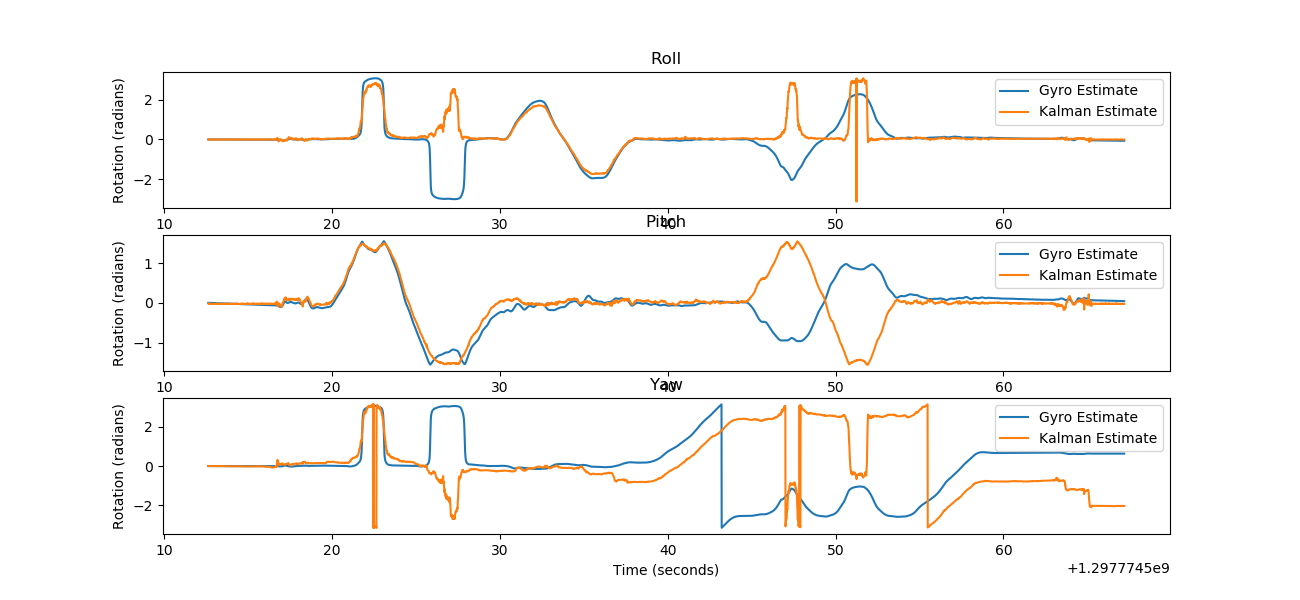
\includegraphics[width=1\textwidth]{rpy_testset13.png}
  \caption{Estimated orientation over time (Test 13)\label{fig:rpy_testset13}}
\end{figure}

\subsection{Panorama Results}

Panoramas are generated using both the vicon ground truth, and the filter output. As expected, the vicon data produced much cleaner results as in figures \ref{fig:panorama1_nocrop} - \ref{fig:panorama9_nocrop}. In some data sets the camera translates at the end of the dataset causing a distortion in the final results, a comparison of the resulting panorama with and without these trailing images are in figures \ref{fig:panorama1_nocrop} and \ref{fig:panorama1}. For completeness, all other figures include the full image set.

Images \ref{fig:panorama1_kalman} to \ref{fig:panorama9_kalman} are panoramas generated from the filtered training data, these are not nearly as clean as the vicon generated panoramas. Images \ref{fig:panorama10_kalman} to \ref{fig:panorama13_kalman} are images generated from the test set, for which no vicon data is available. Therese have varying degrees of success, though in most cases the general form of the room is discernible.

\section{Conclusion}

The Unscented Kalman filter is a decent way of accounting for integration drift during orientation estimation. More work must be done to improve its performance during regular operation. Future work may include adding low pass filters to the gyroscope, and changing the states used by the filter.

\bibliographystyle{alpha}
\bibliography{sample}

\begin{figure}[h]
  \centering
    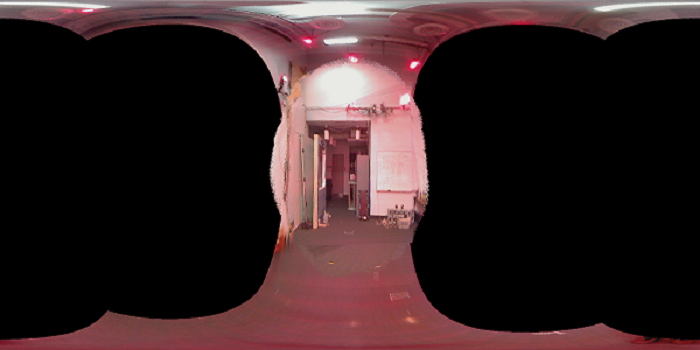
\includegraphics[width=1\textwidth]{PANORAMA1_small.png}
  \caption{Panorama 1 using cropped Vicon data\label{fig:panorama1}}
\end{figure}

\begin{figure}[h]
  \centering
    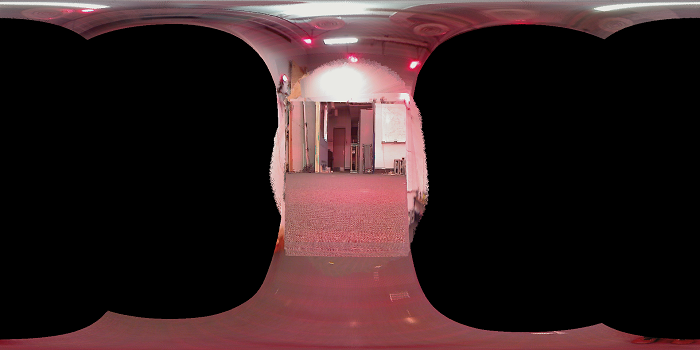
\includegraphics[width=1\textwidth]{PANORAMA1_nocrop_small.png}
  \caption{Panorama 1 using Vicon data\label{fig:panorama1_nocrop}}
\end{figure}

\begin{figure}[h]
  \centering
    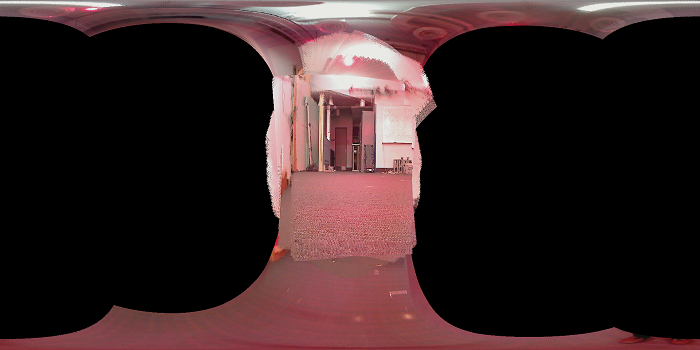
\includegraphics[width=1\textwidth]{PANORAMA2_nocrop_small.png}
  \caption{Panorama 2 using Vicon data\label{fig:panorama2_nocrop}}
\end{figure}

\begin{figure}[h]
  \centering
    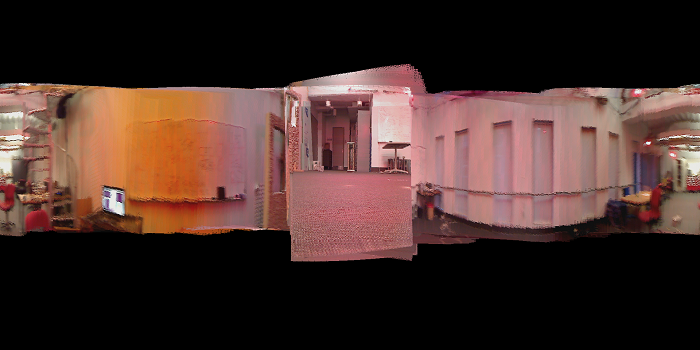
\includegraphics[width=1\textwidth]{PANORAMA8_nocrop_small.png}
  \caption{Panorama 8 using Vicon data\label{fig:panorama8_nocrop}}
\end{figure}

\begin{figure}[h]
  \centering
    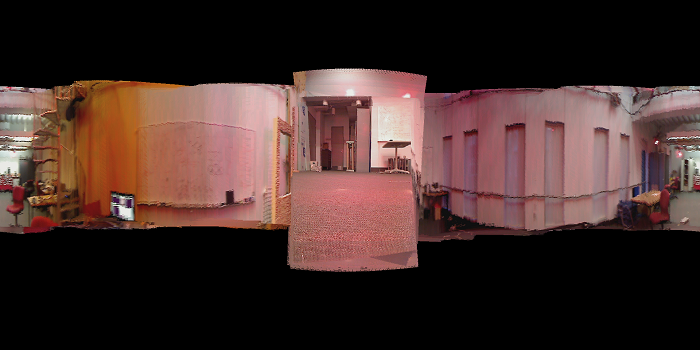
\includegraphics[width=1\textwidth]{PANORAMA9_nocrop_small.png}
  \caption{Panorama 9 using Vicon data\label{fig:panorama9_nocrop}}
\end{figure}

\begin{figure}[h]
  \centering
    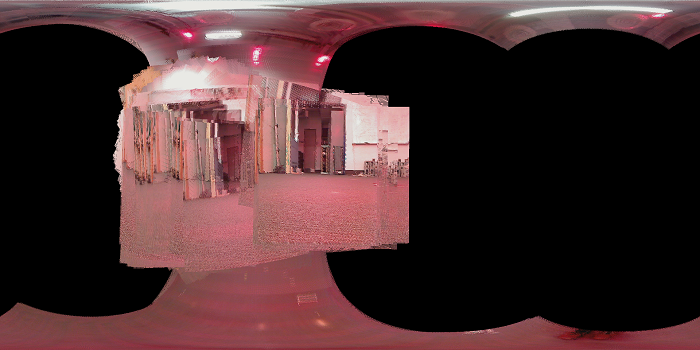
\includegraphics[width=1\textwidth]{pan_trainset1_kalman_small.png}
  \caption{Panorama 1 using Kalman data\label{fig:panorama1_kalman}}
\end{figure}

\begin{figure}[h]
  \centering
    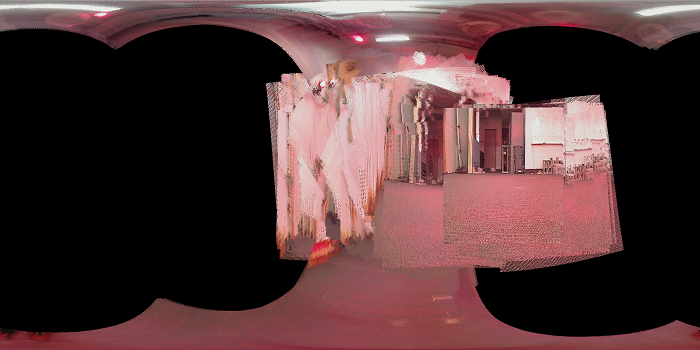
\includegraphics[width=1\textwidth]{pan_trainset2_kalman_small.png}
  \caption{Panorama 2 using Kalman data\label{fig:panorama2_kalman}}
\end{figure}

\begin{figure}[h]
  \centering
    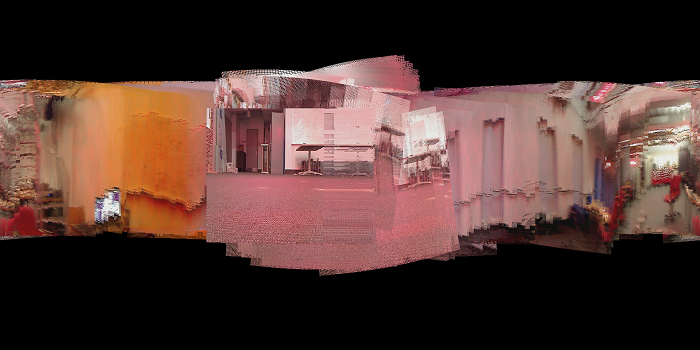
\includegraphics[width=1\textwidth]{pan_trainset8_kalman_small.png}
  \caption{Panorama 8 using Kalman data\label{fig:panorama8_kalman}}
\end{figure}

\begin{figure}[h]
  \centering
    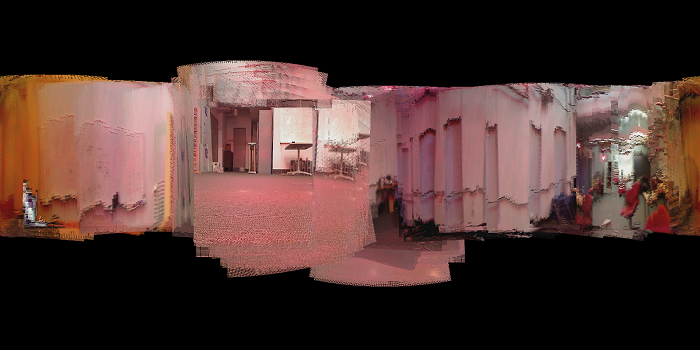
\includegraphics[width=1\textwidth]{pan_trainset9_kalman_small.png}
  \caption{Panorama 9 using Kalman data\label{fig:panorama9_kalman}}
\end{figure}

\begin{figure}[h]
  \centering
    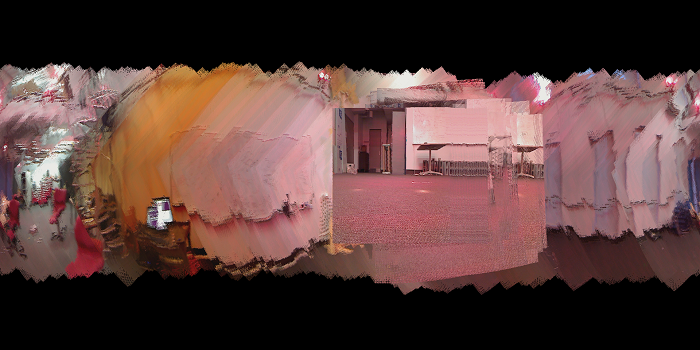
\includegraphics[width=1\textwidth]{pan_testset10_kalman_small.png}
  \caption{Panorama 10 using Kalman data\label{fig:panorama10_kalman}}
\end{figure}

\begin{figure}[h]
  \centering
    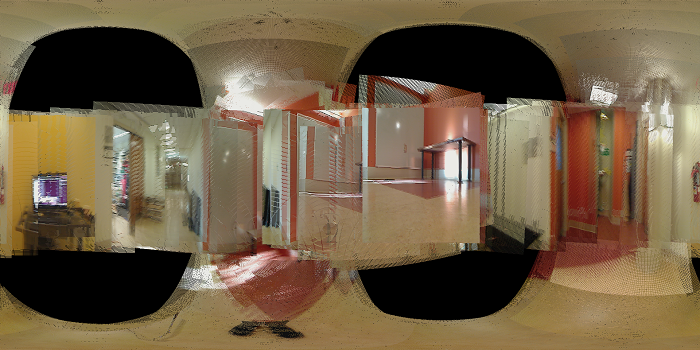
\includegraphics[width=1\textwidth]{pan_testset11_kalman_small.png}
  \caption{Panorama 11 using Kalman data\label{fig:panorama11_kalman}}
\end{figure}

\begin{figure}[h]
  \centering
    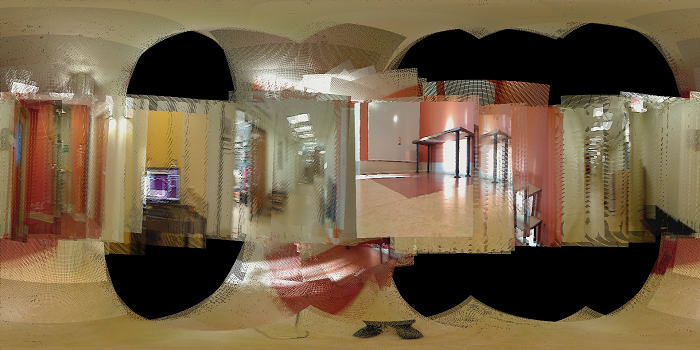
\includegraphics[width=1\textwidth]{pan_testset12_kalman_small.png}
  \caption{Panorama 12 using Kalman data\label{fig:panorama12_kalman}}
\end{figure}

\begin{figure}[h]
  \centering
    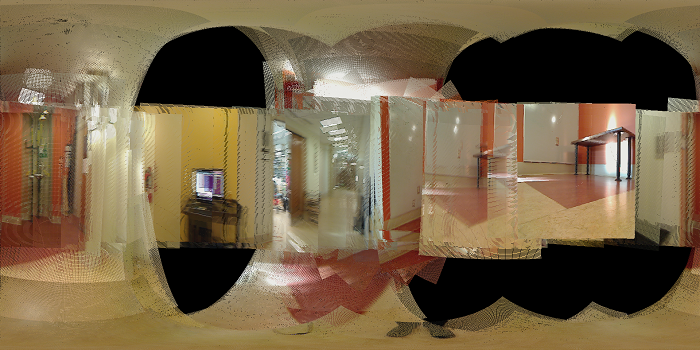
\includegraphics[width=1\textwidth]{pan_testset13_kalman_small.png}
  \caption{Panorama 13 using Kalman data\label{fig:panorama13_kalman}}
\end{figure}

\end{document}